\section{Sprint planning}
After assembling all the tools in Sprint0, we decided to start with the implementation of core modules.
As our understanding of task improved, we were able to come up with user stories from the perspective of user, customer, developer and student.
All user-stories were given to the customer so they can be prioritized. 
All but user-stories concerning our student obligations, like writing project plan, minutes, meetings with supervisor and attending lectures.
Those were mandatory and already added as user-stories of sprint1.
On Monday 02.09.2013. we had the meeting with a customer where we estimated time we need for every user story.
The result of that meeting was the list of the rest of the user-stories for sprin1.
All user stories for finishing our first prototype were on the sprint1 list so we also agreed date for presentation and showing the running demo - Thursday 12.09.2013. 
After that ,at a group meeting, we decoupled user-stories into tasks and we were ready to start with the imlementation of client-server core module.


\subsection{Sprint1 User-stories}

\begin{longtable}{cp{8cm}cc} 
\toprule[1mm]
\textbf{ID} 	& \textbf{Description} 									& \textbf{Est.} & \textbf{Sp.} \\
\hline
\textbf{353} 	& {\bf I as a developer need to make client receive commands from server.} 	& 			& \textbf{4h} \\

\textbf{345} 	& {\bf Customer meeting.} 	& 			& \textbf{6h} \\

\textbf{344} 	& {\bf Team building.} 	& 			& \textbf{9h} \\
				
\textbf{314} 	& {\bf I as a developer need to put �Hello World� project to gitHub and pull it to every group member�s local storage} 	& 	3h	& \textbf{ 4.7h} \\
				& Create folder on gitHub account named "source".	&  &  \\
				& PInstall ADT and Eclipse to our local computers 	&  &  \\
				& Create new Android Project and push it to gitHub 	&  &  \\
				
\textbf{267} 	& {\bf As a user I want to easily download the app from testflight. } 	& 		5	& \textbf{9} \\
				& Set up testflight.	& 2h & 2h \\
				& integrate testflight SDK & 3h & 3h \\
				
\textbf{312} 	& {\bf I as a developer need to make server to be able to listen for clients.} 	& 	25	& \textbf{30} \\
				& Research about server sockets	&  &  \\
				& Implement server listener	&  &  \\
				& Create the moc client. &  &  \\
				& Connect with mock client. &  &  \\
				
\textbf{335} 	& {\bf The server sends one command to one client. } 	& 		4	& \textbf{4} \\

\textbf{336} 	& {\bf The client receives one command } 	& 	2	& \textbf{2} \\

\textbf{334} 	& {\bf The client �plays� one command (white light 10 seconds) } 	& 		4	& \textbf{2} \\

\textbf{327} 	& {\bf As a students we need to attend a meeting with our supervisor. } 	& 		16	& \textbf{16} \\
				& Attend meeting with supervisor week1 (06.09.2013)	&  &  \\
				& Attend meeting with supervisor week2 (13.09.2013)	&  &  \\

\textbf{321} 	& {\bf I as a student need to participate to lectures about team dynamics this week. } 	& 		32	& \textbf{25} \\
				& Course of group dynamics Thu	&  &  \\
				& Summary of course and exchange learned.	&  &  \\
				
\textbf{290} 	& {\bf As a user I want to see the number of connected devices. } 	& 		0.5h	& \textbf{0.5h} \\

\textbf{341} 	& {\bf Integrate TestFlight into application. } 	& 		15h	& \textbf{3h} \\

\textbf{343} 	& {\bf As developer I have to work on Project Plan.} 	& 		12h	& \textbf{12h} \\

\textbf{313} 	& {\bf I as a developer need to establish basic communication protocol between client & server.} 	& 		4h	& \textbf{4h} \\

\textbf{262} 	& {\bf I as a developer need to research TestFlightApp. } 	& 		6h	& \textbf{2.5h} \\
				& Figure out whether to use HockeyApp or TestFlight&  &  \\
				& Research TestFlight	&  &  \\
				
\hline
				& \textbf{SUM:}		&			& \textbf{161}
 \\																			
\bottomrule[1mm]
\caption{User stories selected for Sprint 0. }
\label{tab:sprint0stories}
\end{longtable}

\begin{longtable}{cp{8cm}cc}
\toprule
\textbf{ID} 	& \textbf{Description} 									& \textbf{Est.} & \textbf{Sp.} \\
\hline
\textbf{259} 	& \LaTeX \textbf{template for minutes project plan} 	& 5 			& 4 \\
				& Minutes document \\
				& Report document \\
\hline						
\textbf{245} 	& \textbf{Product and team name} 						& 1 			& 1 \\
				& team name \\
				& product name \\
\bottomrule
\end{longtable}

\section{System Burndown}

\begin{figure}[H]
	\centering
		%\includegraphics[width=10cm]{sprint1/burn_down_sprint1.png}
	\caption{Sprint1 Burn Down Chart}
	\label{fig:sprint1_burn_down_chart}
\end{figure}

\section{Architecture}

Choosing client-server arhitecture was very intuitive to do.
Our project has user application that depends on commands for what to play, on one side, and application that is responsable of detecting and sending commands to that users on the other.
Every aplication(user) have to be either one or another. 

Write about Android NSD, create class diagram, 


\begin{figure}[!t]
	\centering
		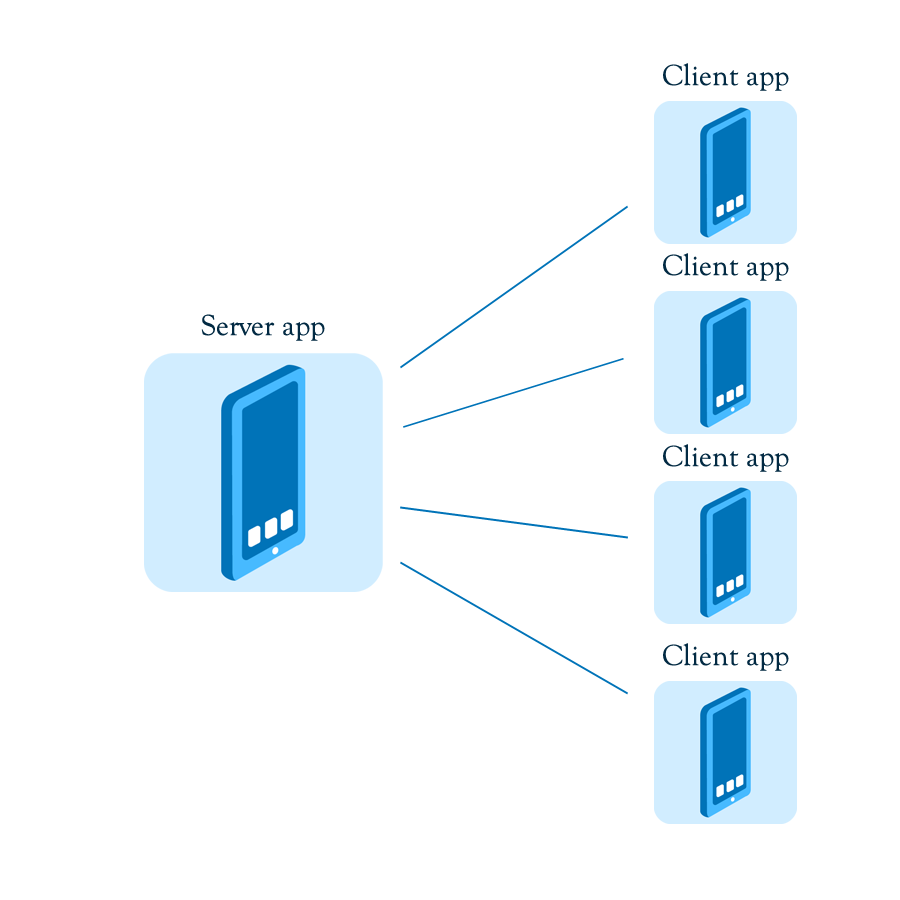
\includegraphics[width=16cm]{sprint1/arhitecture.png}
	\caption{Sprint1 Arhitecture}
	\label{fig:sprint1_arhitecture}
\end{figure}

\section{Implementation}
\section{Testing}
\section{Occurring risks}
\section{Retrospective}
\subsection{Pros}
\subsection{Cons}
\section{Evaluation}